\documentclass[conference]{IEEEtran}
\IEEEoverridecommandlockouts
% The preceding line is only needed to identify funding in the first footnote. If that is unneeded, please comment it out.
\usepackage{cite}


\usepackage{amsmath,amssymb,amsfonts}
\usepackage{algorithmic}
\usepackage{graphicx}
\usepackage{textcomp}
\usepackage{xcolor}
\usepackage{url}
\def\BibTeX{{\rm B\kern-.05em{\sc i\kern-.025em b}\kern-.08em
    T\kern-.1667em\lower.7ex\hbox{E}\kern-.125emX}}
\begin{document}

\title{Panoramic Video Stitching with Small Overlap\\
%{\footnotesize \textsuperscript{*}Note: Sub-titles are not captured in Xplore and
%should not be used}
%\thanks{Identify applicable funding agency here. If none, delete this.}
}

\author{\IEEEauthorblockN{Chaoyu Xie and Xuejin Chen}
\IEEEauthorblockA{\textit{University of Science and Technology of China} \\
%\textit{name of organization (of Aff.)}\\
%Anhui, China \\
xcy12345@mail.ustc.edu.cn, xjchen99@ustc.edu.cn}
%\and
%\IEEEauthorblockN{Xuejin Chen}
%\IEEEauthorblockA{\textit{University of Science and Technology of China} \\
%\textit{name of organization (of Aff.)}\\
%Anhui, China \\
%xjchen99@ustc.edu.cn}
%\and
%\IEEEauthorblockN{3\textsuperscript{rd} Given Name Surname}
%\IEEEauthorblockA{\textit{dept. name of organization (of Aff.)} \\
%\textit{name of organization (of Aff.)}\\
%City, Country \\
%email address}
%\and
%\IEEEauthorblockN{4\textsuperscript{th} Given Name Surname}
%\IEEEauthorblockA{\textit{dept. name of organization (of Aff.)} \\
%\textit{name of organization (of Aff.)}\\
%City, Country \\
%email address}
%\and
%\IEEEauthorblockN{5\textsuperscript{th} Given Name Surname}
%\IEEEauthorblockA{\textit{dept. name of organization (of Aff.)} \\
%\textit{name of organization (of Aff.)}\\
%City, Country \\
%email address}
%\and
%\IEEEauthorblockN{6\textsuperscript{th} Given Name Surname}
%\IEEEauthorblockA{\textit{dept. name of organization (of Aff.)} \\
%\textit{name of organization (of Aff.)}\\
%City, Country \\
%email address}
}

\maketitle

\begin{abstract}
Video stitching remains a challenging problem in computer vision. In this paper, we propose a novel method to stitch multiple videos which have small overlapped regions.
Our algorithm consists of three steps: (1) spherical projection of the input video frames based on camera calibration, (2) edge detection and edge-guided feature matching for frame registration, and (3) seam optimization to eliminate distortions and ghosts in the composited panoramic videos. 
%
The experimental results and user studies 
demonstrate that out method is robust to videos that have small overlapped regions and produces more visually pleasing panoramic videos than state-of-the-art techniques.
\end{abstract}

\begin{IEEEkeywords}
video stitching, panorama, overlap, edge detection
\end{IEEEkeywords}

\section{Introduction}
\label{sec:intro}

Video stitching is the process to composting a panoramic video from several videos that have overlap regions. %The holy goal of video stitching is to acquire a large view video that looks as natural as possible. 
As a result of the widespread
use in security monitoring, virtual reality and medical image
analysis, video stitching has become a hot topic in recent years.

Most video stitching techniques \cite{zheng2008stitching, guo2016joint, Jiang_2015_CVPR_Workshops, nie2018dynamic} require videos that overlap with
their neighboring videos by a large margin.
Under this case, sufficient feature points can be detected and matched to compute the transformation between adjacent views.
There are also lots of commercial software, such as VideoStitch Studio \cite{videostitching}, AutoPano \cite{autopano}, to composite panoramic images or videos by computing transformations between neighboring views based on feature detection and matching.
When the overlap between adjacent views is relatively small, these methods and software fail to get enough feature matches, thus can not stitch the videos together.

%For example, a typical scenario we envision is: six cameras fixed on a tripod. 
Fig. \ref{fig:equipment} shows a typical panorama capturing device that consists of six cameras. 
Although the field of view (FOV) of the cameras is very large, the overlap between the cameras is small. 
Stitching such six videos is very challenging due to two
major reasons. First, it is difficult to find enough feature points and matches in small overlapping regions between videos. Second, structure distortion and ghost of moving objects in the scene are likely to occur without enough overlap to correct these artifacts. 

In this paper, we propose an edge-guided approach to stitch videos that have small overlaps by looking for sufficient matches in a local region guided by edges. 
%Different from the period work \cite{Jiang_2015_CVPR_Workshops}, we mainly focus on video stitching which has a small overlapping area.
%
Our algorithm first projects the input videos into spherical coordinate systems based on pre-calibrated camera intrinsics. 
Then, scene edges are extracted and guide according to the edge we mesh these video into grids frame by frame.
And calculating the homography matrix of each gird. Finally, we update seam and produce a panoramic video.
Fig. \ref{fig:res} shows the video stitching process presented in this paper.

\begin{figure}[t]
\centering
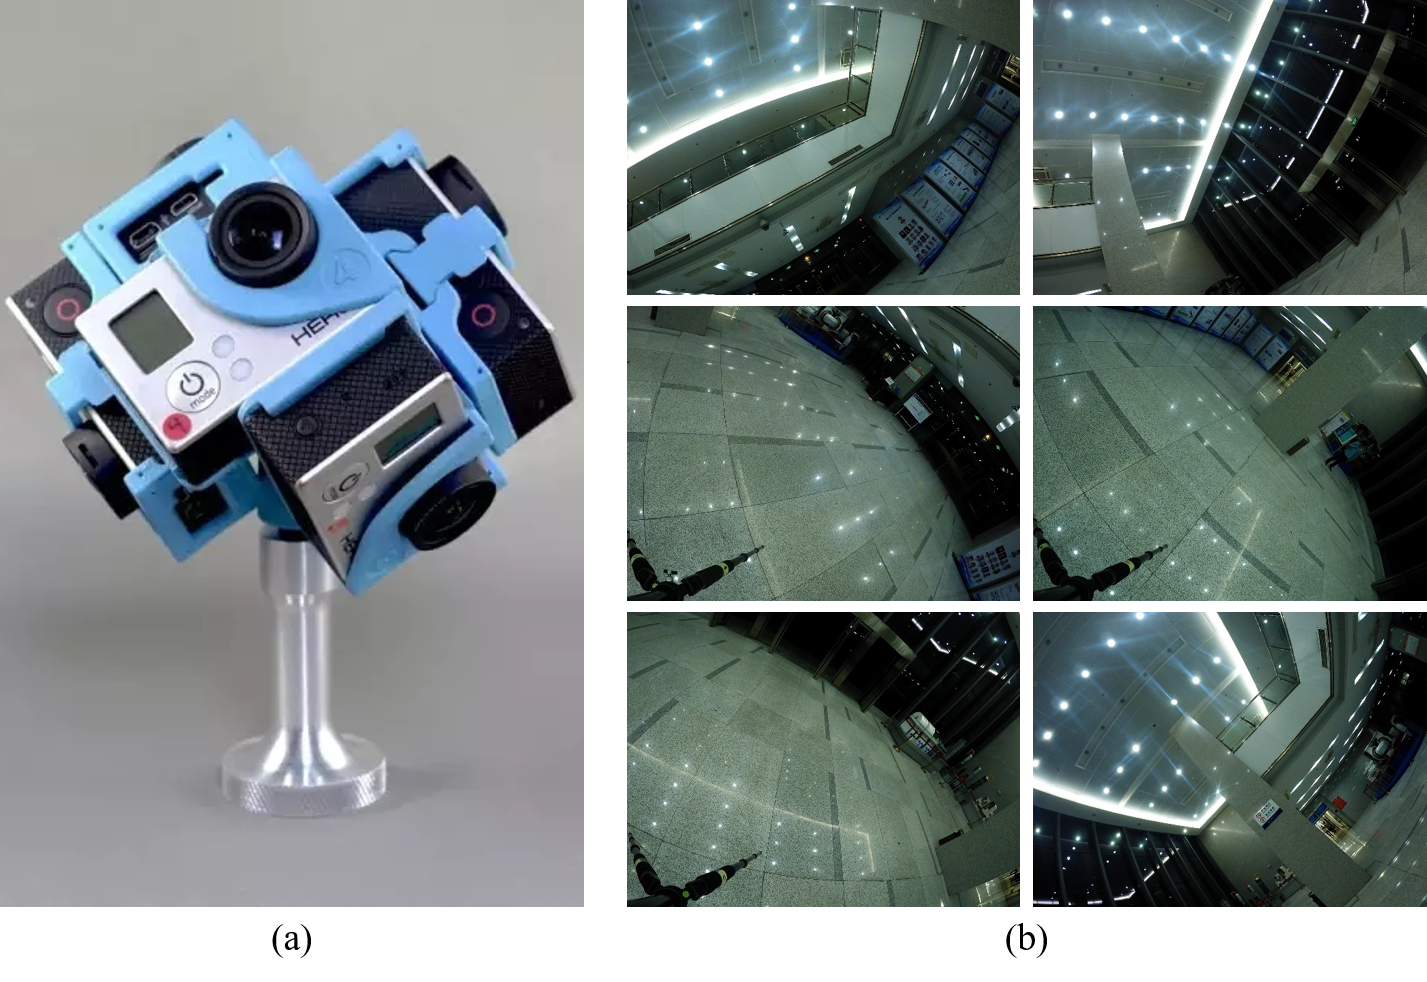
\includegraphics[scale=0.36]{picture34.png}
\caption{A six-camera cube-shape device to capture videos (a), and six frames captured by the device (b). Even with large field-of-view (FOV) of each camera, neighboring videos have relatively small overlaps. }
\label{fig:equipment}
\end{figure}

\begin{figure*}
\centering
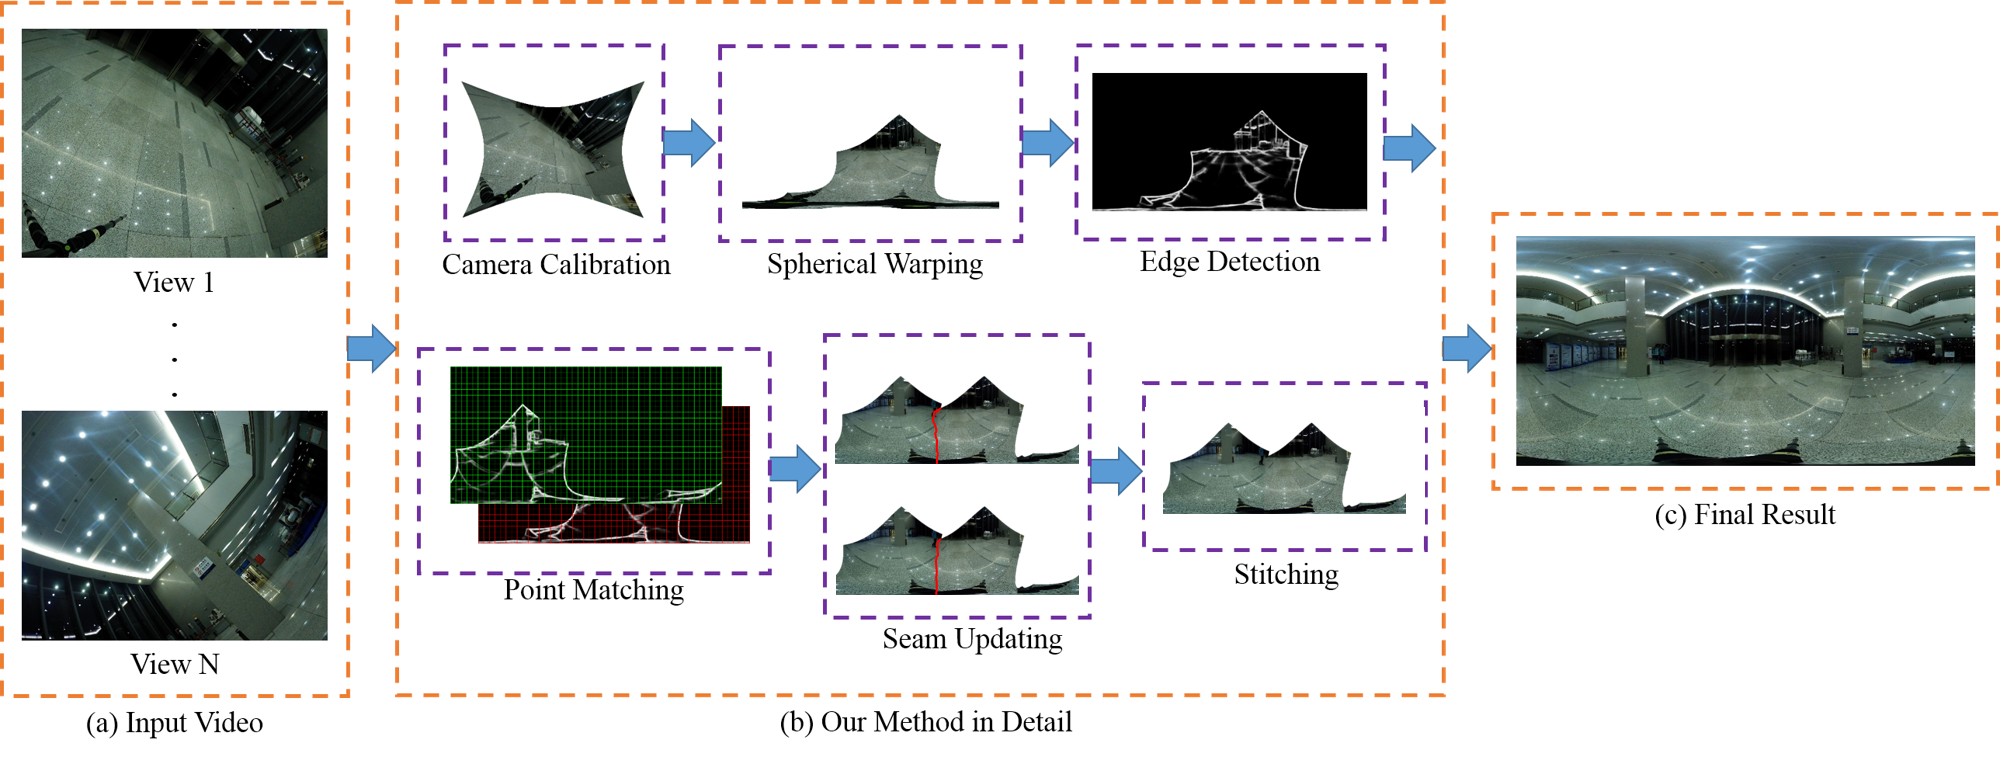
\includegraphics[scale=0.54]{picture49.png}
\caption{The pipeline of our video stitching algorithm. First, we pre-process the video data, such as calibrating the camera
and projecting the video frame into spherical coordinates. Second, we detect the edge of each spherically
warped frame and re-calculate
homography matrix in every grid. Third, updating seam and stitching the videos to produce a panoramic video.}
\label{fig:res}
\end{figure*}

\section{Related work}
\label{sec:related}

In this section, we briefly review the most related works in image stitching and video stitching.


{\bf Image Stitching.} Image stitching is a well-studied, yet still active research 
area \cite{paragios2006handbook, brown2007automatic,hartley2003multiple,lin2011smoothly, chang2014shape, zaragoza2013projective,lin2015adaptive,zhang2014parallax, gao2013seam, agarwala2004interactive,gao2011constructing}. 
Early methods adopt a single homography to align images.
However, a single homography is valid only when the cameras' optical center are aligned and only rotations exist between cameras, or the captured scene is planar in 3D \cite{hartley2003multiple}. 
Otherwise, there is parallax between the images, and artifacts such as structure distortion and ghosts occur in the composition. 
To solve the parallex problem, two types of stitching strategies have been proposed, including warp-based approaches \cite{lin2011smoothly, chang2014shape, zaragoza2013projective} and seam-driven approaches \cite{zhang2014parallax, gao2013seam, agarwala2004interactive}. 
In the warp-based category, 
Gao \textit{et al.} proposed to use two homographies to model outdoor scenes roughly by two planes (ground plane and distant plane) \cite{gao2011constructing}.
Zaragoza \textit{et al.} proposed an as-projective-as-possible (APAP) mesh deformation that warps
images by following a global projective transformation and allows local non-projective 
deviations \cite{zaragoza2013projective}.
Chang \textit{et al.} proposed a shape-preserving half-projective (SPHP) method
to correct distortions in non-overlapping regions \cite{chang2014shape}. 
Lin \textit{et al.} proposed Adaptive As-Natural-As-Possible (AANAP) 
which is based on APAP but computes the warping fully automatically \cite{lin2015adaptive}.
In the seam-driven category, Agarwala \textit{et al.}
proposed photomontage that composites a photograph by
cutting and stitching multiple photographs seamlessly \cite{agarwala2004interactive},
while Zhang and Liu looked for a homography that leads to a
minimum energy seam to stitch large-parallax images \cite{zhang2014parallax}.
In addition, several freewares and commercial software, such as AutoStitch, Microsoft’s Image Compositing Editor, and Adobe's Photoshop CS6 mosaicing feature, are available for performing image stitching.




\noindent{\bf Video Stitching.} Compared to image stitching, video stitching received much less attention. 
Moving objects in overlapped regions become the most challenging factor for video stitching.
%On the other hand, the complexity of video stitching algorithm is very high.
%
According to different camera settings, various approaches have been proposed. In general, these methods can be divided into two categories: 
stitching methods with fixed cameras \cite{zheng2008stitching, he2010panoramic, Jiang_2015_CVPR_Workshops, perazzi2015panoramic, li2015efficient} 
and stitching methods with moving cameras \cite{lin2016seamless, guo2016joint, nie2018dynamic}. 
%
In the category with fixed cameras, Zheng \textit{et al.} stitched the videos frame by frame without considering temporal relationship between video frames \cite{zheng2008stitching}.
Jiang \textit{et al.} proposed spatial-temporal content-preserving warping (STCPW) to eliminate small deviations \cite{Jiang_2015_CVPR_Workshops}.
In the category with moving cameras, 
Lin \textit{et al.} proposed a method for independently moving mobile devices.
They recovered 3D camera paths and a sparse set of 3D scene points to stitch videos \cite{lin2016seamless}.
Guo \textit{et al.} calculated both inter
motions and intra motions, then calculated camera paths, and finally stitching them together \cite{guo2016joint}.
Nie \textit{et al.} distinguish right and false matches \cite{nie2018dynamic} to stitch videos more robustly. 
One common thing among all these methods is that sufficient overlaps between the input videos cameras are required. 
However, this is not a typical case in real applications. 
In comparison, we solve a more challenging case that the videos to be stitched have very small overlaps.

\section{OUR METHOD}
\label{sec:ourmethod}

Fig. \ref{fig:res} shows the pipeline of our video stitching algorithm.
We calibrate each camera offline to get the intrinsic parameters of each camera. 
Given $N$ videos with fixed order, we first rectify each video into a common image plane to remove tangential and radial distortions.
Then we project the rectified video frames into spherical coordinate system (see details in Sec. \ref{ssec:Pre-prepared}). 
Edges are extracted from each frame.
Each frame is divided into regular grids and we calculate homography matrix in each grid. 
Then matching the points in overlapped region which is described in Sec. \ref{ssec:edge-detection}. 
The third step is stitching them into a panoramic video according to the spatial-temporal information, as described in Sec \ref{ssec:stitching}.

\subsection{Frame Rectification and Warping}
\label{ssec:Pre-prepared}

Panorama cameras typically capture images with a wide FOV with radial distortions, as shown in Fig.~\ref{fig:ori_cal_pro}(a).
In order to get more matching points and more accurate image alignment, we rectify the input videos and project them into a spherical coordinate system.
%Pre-process for video stitching composes of two parts, the one is calculating the parameters of the cameras, the other is projecting the video into a new coordinate system. The parameters of a camera consist intrinsics and extrinsics. 
We use the method proposed in \cite{zhang2000flexible} to calculate the intrinsic parameters of each camera, and compute the rotation matrix according to the device setting. 
%
The radial distortions can be eliminated based on the camera intrinsic matrix, as Fig.~\ref{fig:ori_cal_pro}(b) shows.
%
Then we convert each rectified video into spherical coordinates.
Let $\mathbf{x}_{s} = (x_{s},y_{s})^T$ be a point on the spherically
warped frame $F$, its corresponding point $\mathbf{x} = (x, y)^T$ on rectified frame $F_r$ is calculated as:
\begin{equation}
\begin{aligned}
\theta =\left(x_{s}-x_{c}\right) &/ f , \varphi =\left(y_{s} -y_{c}\right) / f \\
x'=sin\theta \cos\varphi, y'&=\sin\varphi, z'=\cos\theta \sin\varphi \\
\left[ \begin{array}{l}{\hat{x}} \\ {\hat{y}} \\ {\hat{z}}\end{array}\right]&=\textbf{R} \left[ \begin{array}{l}{x^{\prime}} \\ {y^{\prime}} \\ {z^{\prime}}\end{array}\right]\\
x&=f\frac{\hat{x}}{\hat{z}}+x_c\\
y&=f\frac{\hat{y}}{\hat{z}}+y_c,
\end{aligned}
\end{equation}
where $\textbf{R}$ stands for the extrinsic rotation matrix of the camera, $x_c$ and $y_c$ stands for the image center of $F$, $f$ stands for the focal length of the camera.
Fig. \ref{fig:ori_cal_pro}(c) shows the process of frame rectification and spherical warping. 

\begin{figure}[t]
\centering
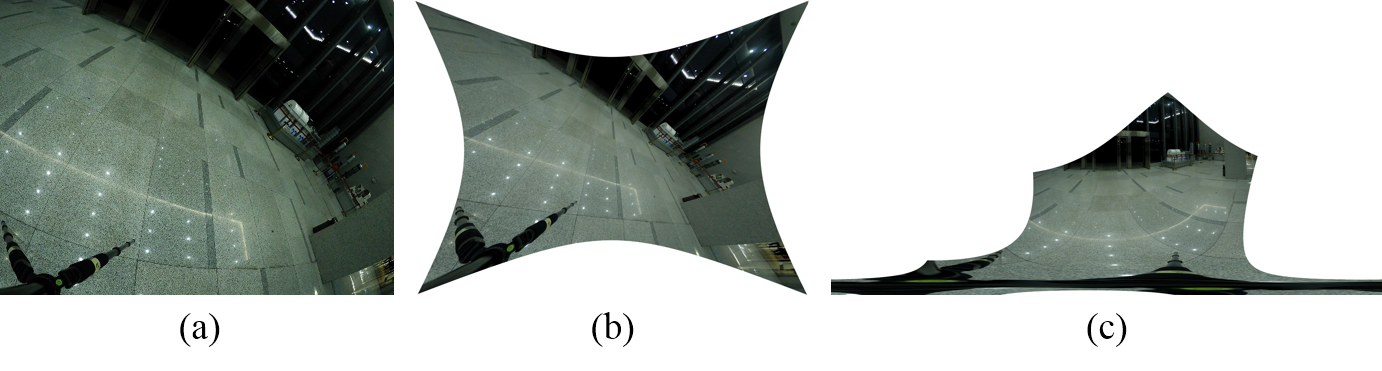
\includegraphics[scale=0.23]{picture40.png}
\caption{An example frame captured by the camera (a), and the rectified image (b) to eliminate radial distortion. Then the rectified image is converted to spherical coordinate (c).}
\label{fig:ori_cal_pro}
\end{figure}




\subsection{Edge-Guided Video Alignment}
\label{ssec:edge-detection}

Since neighboring videos overlap in a very small area, it is not easy to find enough matches of feature points, especially when there a textureless region or repeated patterns in the scene. 
In order to resolve the ambiguity in feature matching, we propose to search for matching points along edges.
%
To detect primary edges in the scene, we use holistically-nested edge detection (HED) \cite{xie2015holistically}. 
Then we divide each frame into $m \times n$ regular girds, where $m=25$ and $n=50$ in our experiments.
%
For each grid in the overlapped region between two neighboring frames, we compute its homography by looking for a least four pairs of feature points.
%
For each pixel on the edges in the grid, we look for its nearest pixel on the edges in its neighboring frame as matching pairs.  
%
According to the obtained matching point pairs $\mathbf{a}$ to $\mathbf{a}'$ in two neighboring frames, we compute the homography $\mathbf{H} \in \mathbb{R}^{3 \times 3}$ by solving a group of linear equations 
%Let $\textbf{a} = [i \ j]^T$ and $\textbf{a}' = [i' \ j']^T$ be matching points across overlapping frames $F_l$ and $F_r$. 
%A projective warp or homography aims to map $\textbf{a}$ to $\textbf{a}'$ following the relation:
\begin{equation}
\widetilde{\textbf{a}}' \sim \mathbf{H} \widetilde{\textbf{a}},
\end{equation}
where $\widetilde{\mathbf{a}}=(x,y,1)^{T}$ is the homogeneous coordinate of a 2D point $(x,y)^{T}$.  
%According to the matrix, the points can be projected to the correct region.
There maybe some grids where no edge is found. 
For these grid, we calculate its homography matrix according to its four neighboring grids. 
Let $\textbf{H}_i$ be the homography matrix in grid $i$.
If there is no points are detected in grid $i$, its homography matrix $\textbf{H}_{i}$ can be calculated as:
\begin{equation}
\textbf{H}_{i} = \frac{1}{4}\left(\textbf{H}_{il}+\textbf{H}_{ir}+\textbf{H}_{iu}+\textbf{H}_{id}\right),
\end{equation} 
where $\textbf{H}_{il}$, 
$\textbf{H}_{ir}$, 
$\textbf{H}_{iu}$, 
$\textbf{H}_{id}$ 
denote four homography matrices of grid 
$i$.
Fig. \ref{fig:p8} illustrates the alignment process.
With our edge-guided image alignment, the scene structures and object boundaries are well aligned. 




\begin{figure}[!htpb]
\centering
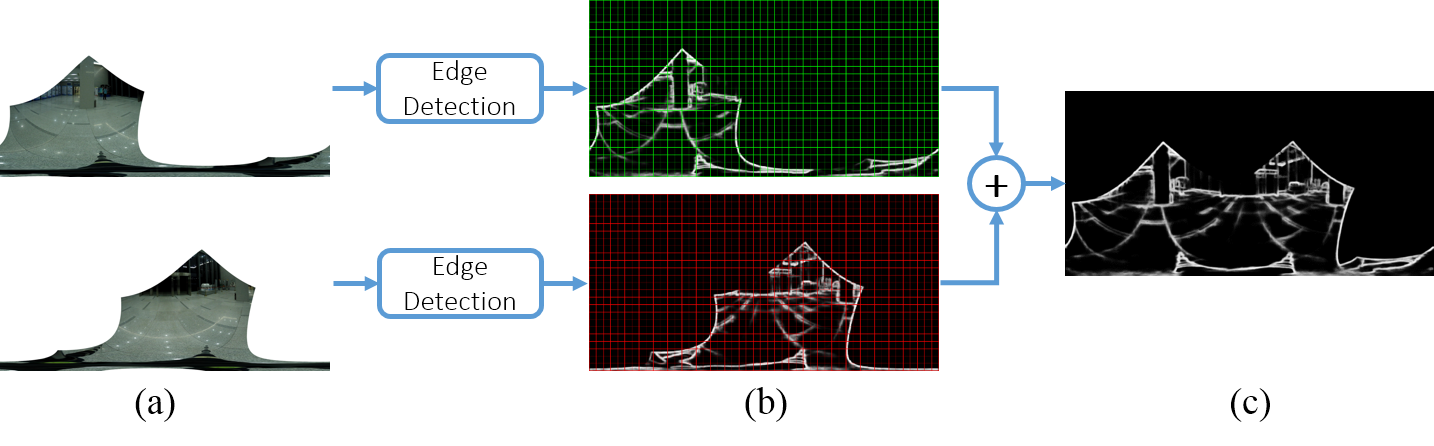
\includegraphics[scale=0.35]{picture41.png}
\caption{For two neighboring frames that are converted to a spherical coordinate system, edges are first extracted for each frame (a). Then by dividing each frame into grids,  we compute the homography matrix for each grid by looking for matching point pairs on the extracted edges (b).
Finally the two frames are aligned according to the computed homography matrices on the overlapping grids. The scene edges are well aligned.}
\label{fig:p8}
\end{figure}

\subsection{Seam Updating and Stitching}
\label{ssec:stitching}

While our edge-guided alignment process well preserves scene structures and avoids edge distortions, it does not eliminate ghosts when there is a moving object through the overlapped region.
To stitch the two videos seamlessly, we adopt the overlaying strategy as in \cite{he2016parallax}. 
Firstly, we search a seam in the overlapping region using graphcut algorithm \cite{boykov2004experimental}, as shown in Fig. \ref{fig:p24}(b) in red line.
%\textcolor{red}{(Add grid illustration and explain more how do you generate the seams.)} 
Secondly, using $g_{i0}$ as the original gradient of pixel $p_i$ in the present seam, and using $g_{it}$ as the gradient of pixel $p_i$ in time $t$. To calculate whether the gradient
of pixels have a big change, we use the following rule:
\begin{equation}
\textit{C}_{t}=\{p_{i}|\frac{g_{it}-g_{i0}}{g_{i0}}>\sigma\}
\end{equation}
where $\sigma=1.0$ in our experiments.
If the total pixel number in $\textit{C}_t$ is bigger than $0.4N_{seam}$, which means that there is likely a new object moving through the overlapping region. 
Here, $N_{seam}$ is the total pixel number of the seam. 
And then, the seam will be updated. We use graphcut algorithm but remove those points which are in $C_t$ to update seam at time $t$. 
Fig. \ref{fig:p24}(c) shows the points which are removed in yellow color.
Otherwise, we continue to use the previous seam.
%\textcolor{red}{explain how do you update the seam. Update seam of which frame? which time? }
Finally, to stitch the video well, we use linear blending method.
Fig. \ref{fig:p24} shows the method.
\begin{figure}[h]
\centering
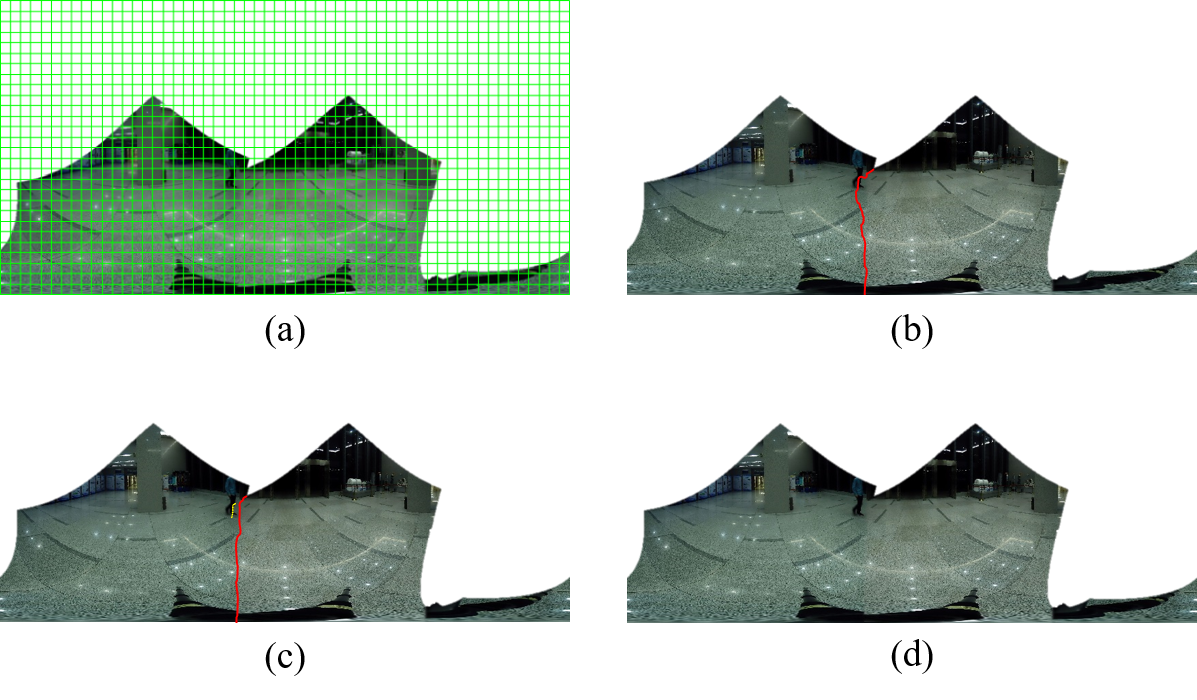
\includegraphics[scale=0.42]{picture50.png}
\caption{(a) shows an aligned frame in green grids and the origin seam in red line (b), (c) shows the updating seam in red line and removed points in yellow color, (d) shows the final fused image.}
\label{fig:p24}
\end{figure}

\section{RESULT}
\label{sec:result}

Since there is no publicly available video stitching benchmark data, we evaluate the proposed method on the 
videos which we captured.  The video datasets are captured by six fixed cameras (Gopro Hero4 Black) with different views which are synchronized. 
These videos are both captured by same type cameras and they are 1440p (1920 $\times$ 1440) at 24 fps.
Because the overlapped region is very small, lots of method we listed in Sec. \ref{sec:related} failed to stitch them together.
The compared methods include APAP and commercial software AutoPano. The video data used in APAP method in this paper was pre-processed. We compare the result as image stitching on each frame firstly.
We randomly select one frame on image stitching. Fig. \ref{fig:pic17} shows the result of APAP, AutoPano and ours. 
From Fig. \ref{fig:pic17} we can see the result of APAP 
destroys the structure of buildings severely, such as the pillar and the light. There are severe ghosts around pillar and light.
As for commercial software, it also can not stitch the image well, such as the pillar have ghosts and the structure of light breaks from the middle, 
but our method keeps the structure well, and has less ghost than the others.

For comparison of moving object through overlapped region, we compare the result of APAP, AutoPano and ours. Fig. \ref{fig:pic15} 
illustrates frames where an object is moving through the overlapped region and the background remains still. 
We select three consecutive frames for comparison. In Fig. \ref{fig:pic15}, APAP and AutoPano have severe ghosts around the walking person in the panoramic video. 
The man's body is distorted in AutoPano method. However, using our proposed method, the man's body is kept well. 
Fig. ~\ref{fig:more1}, Fig. ~\ref{fig:more2} show more comparisons of our method and others.
\begin{table}[!htpb]
\caption{MOS of three algorithms}
\label{tab1:table1}
\centering
\begin{tabular}{c|c|c|c}
\hline
Method& AutoPano& APAP& Ours\\
\hline
MOS& 6.36& 4.62& \bf{7.65}\\
\hline
\end{tabular}
\end{table}
\begin{figure}[!htpb]
\centering
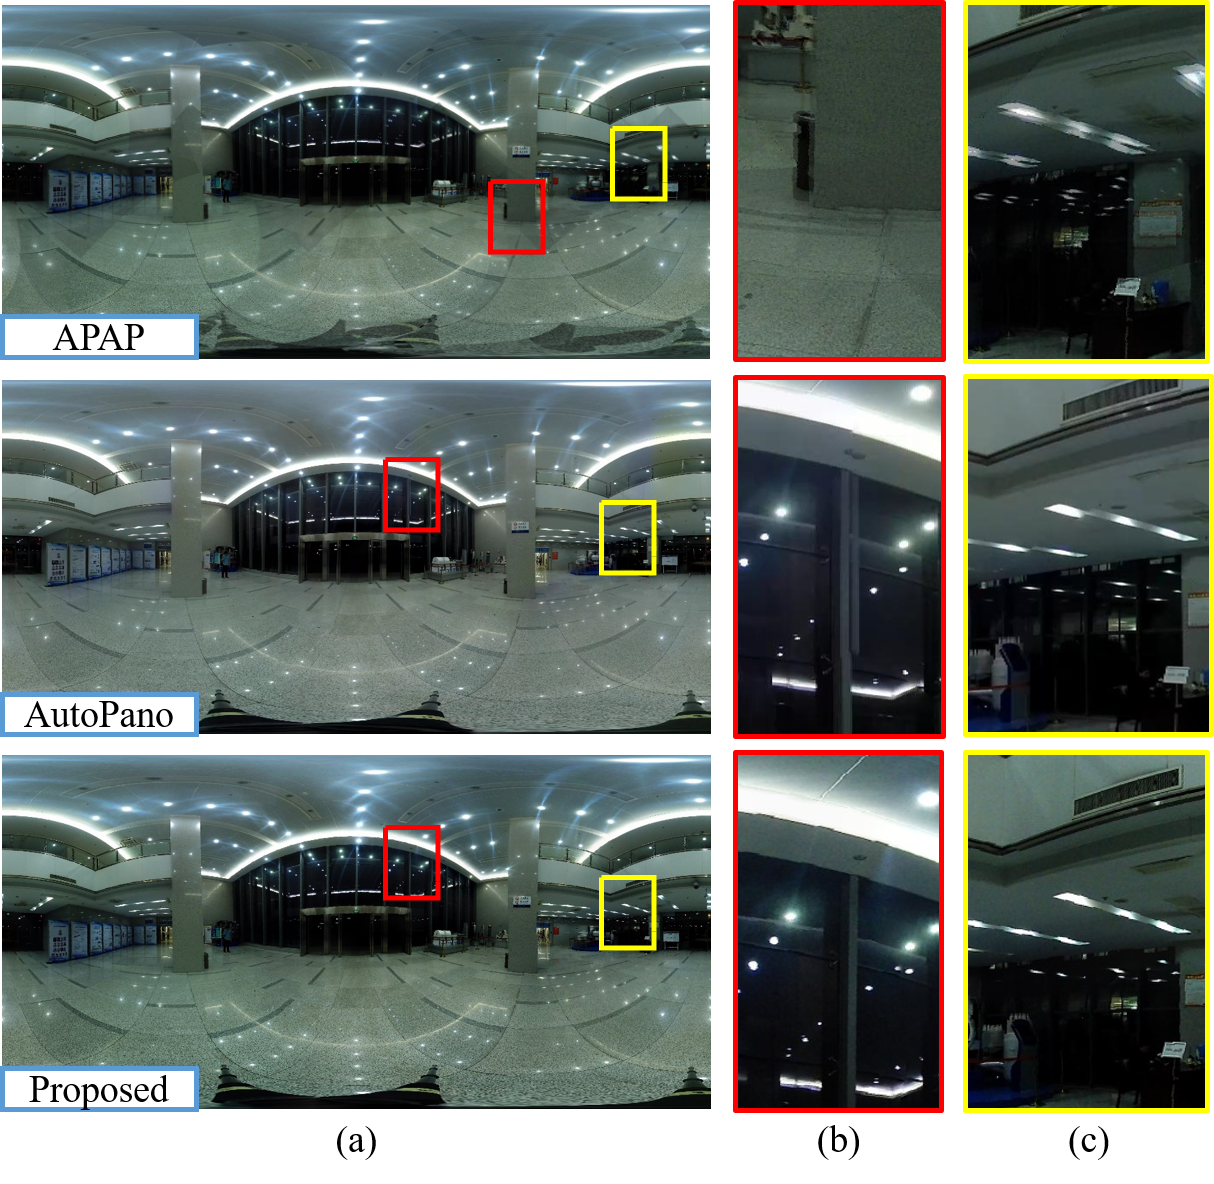
\includegraphics[scale=0.415]{picture35.png}
\caption{Comparisons with APAP, AutoPano and our method. From left to right: (a) one of the stitched frames, (b) enlarged views of local
detail in red box, (c) enlarged views of local detail in yellow box.}
\label{fig:pic17}
\end{figure}
\begin{figure}[!htpb]
\centering
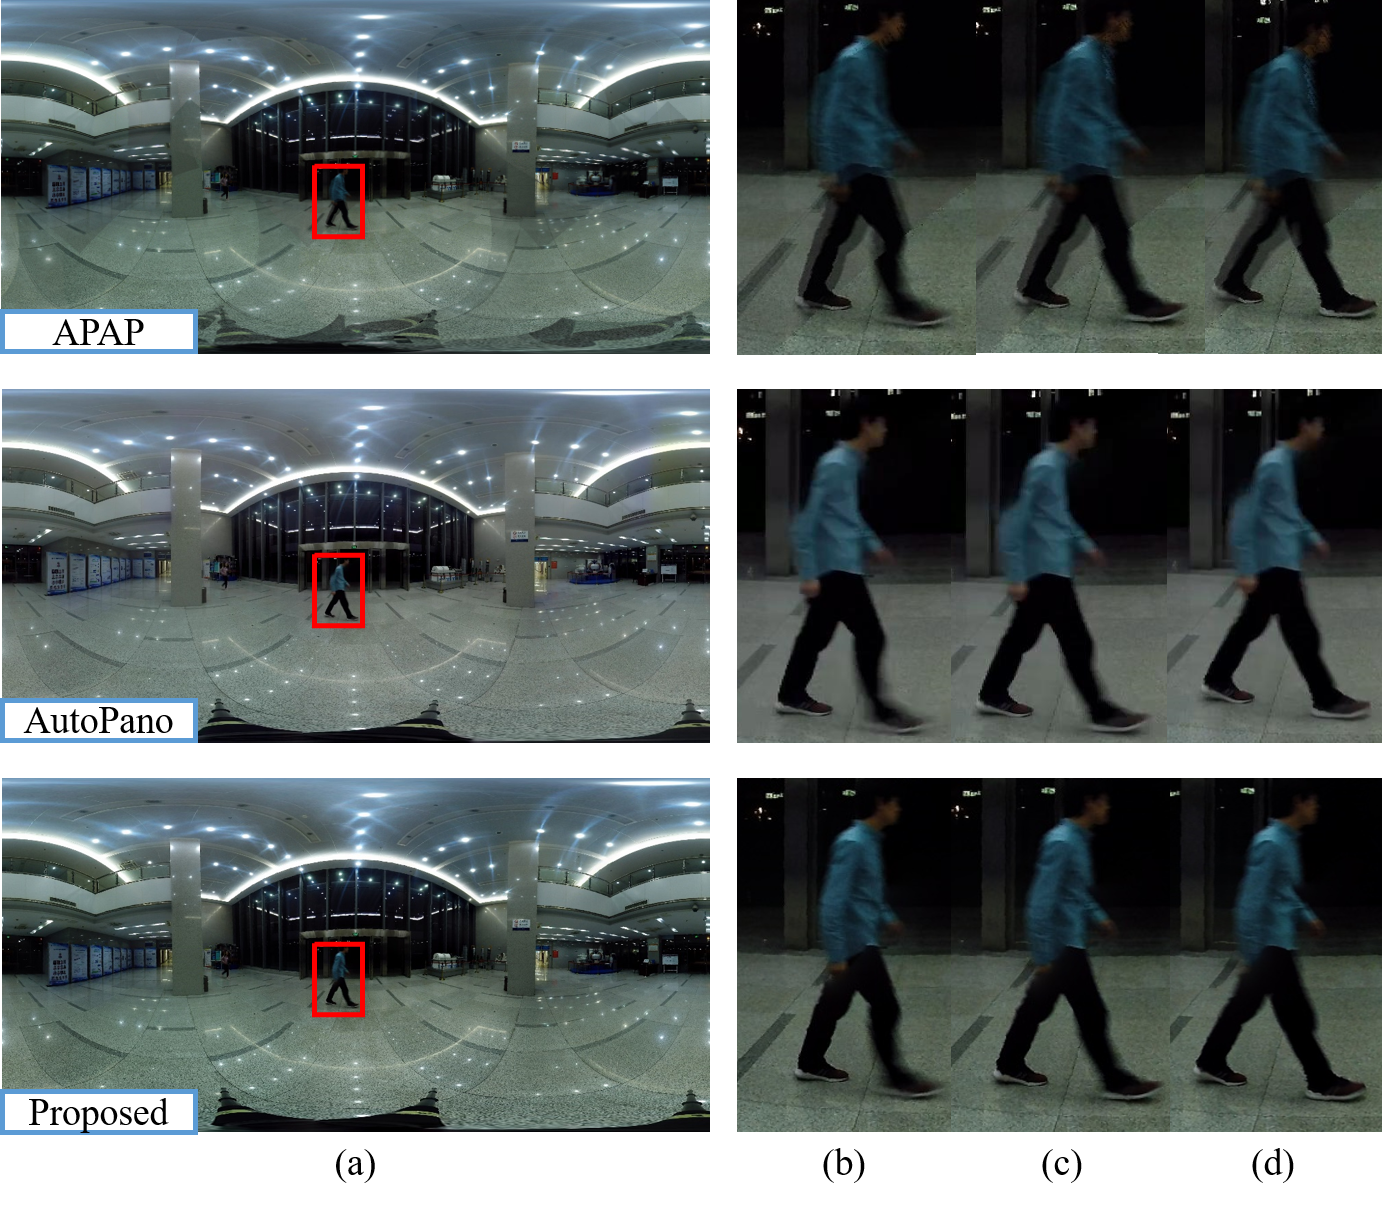
\includegraphics[scale=0.36]{picture36.png}
\caption{Comparisons with APAP, AutoPano and our method when there is an object moving in the overlapped region. From left to right: (a) one of the stitched frames, (b) enlarged views of local
detail in frame $t_1$, (c) enlarged views of local detail in frame $t_2$, (d) enlarged views of local detail in frame $t_3$.}
\label{fig:pic15}
\end{figure}

In order to evaluate the performance of our algorithm, we made a user test interface. The interface shows the results of APAP, AutoPano and our method simultaneously.
We use mean opinion score (MOS) to evaluate the panoramic video. We use 1-10, 10 integers to represent the quality of the video, 
1 represents the worst quality of the video, 10 represents the best quality of the video, and the method of calculating MOS is as follows:
\begin{equation}
{\rm MOS}=\frac{\sum^{N}_{n=1}{R_n}}{N}
\end{equation}
where $N$ stands for the number of people scoring each method and $R_n$ stands for a user's score for each type of video. We take $N=150$ in this experiment.
In the user study, 50 users use interface to score the videos. The videos show on the interface according to the rules: (1) the video groups were random and 
(2) the display order of three methods of one video group was also random.
And then we calculated MOS for each method. Table \ref{tab1:table1} shows the comparison. The MOS of our method is much higher than the others.

\section{CONCLUSION}
\label{sec:conclusion}

In this paper, we proposed a new method to stitch videos which have a small overlapped region. We pre-process the video data, such as calibrating the camera and projecting the video frame into spherical
coordinates. We detect the edge of each spherically warped frame and re-calculate homography matrix in every grid. Using the time domain information to produce panoramic videos. 
Experimental results show that our approach achieves a better panoramic video than state-of-the-art ones. Our algorithm improves image alignment accuracy and reduces artifacts caused by
moving objects. In the future, we would like to speed up our algorithm.

\bibliographystyle{IEEEbib}
\bibliography{refs}
\begin{figure}[!htpb]
\centering
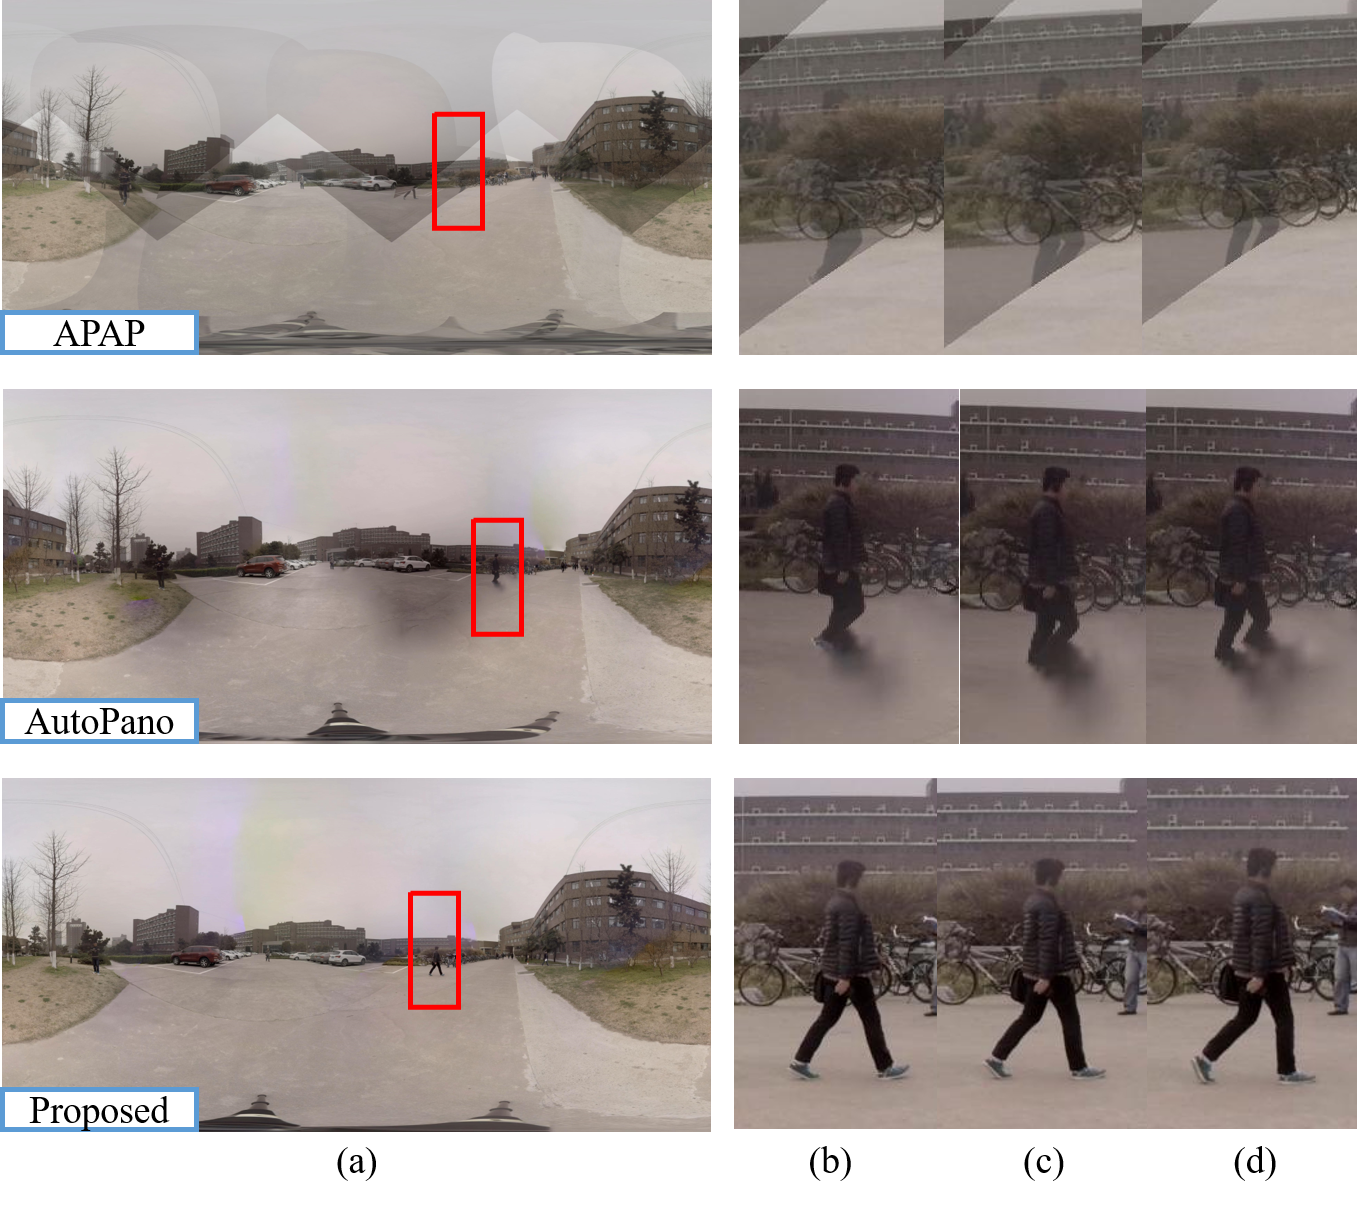
\includegraphics[scale=0.38]{picture37.png}
\caption{Comparisons with APAP, AutoPano and our method when there is an object moving in the overlapped region. From left to right: (a) one of the stitched frames, (b) enlarged views of local
detail in frame $t_1$, (c) enlarged views of local detail in frame $t_2$, (d) enlarged views of local detail in frame $t_3$.}
\label{fig:more1}
\end{figure}
\begin{figure}[!htpb]
\centering
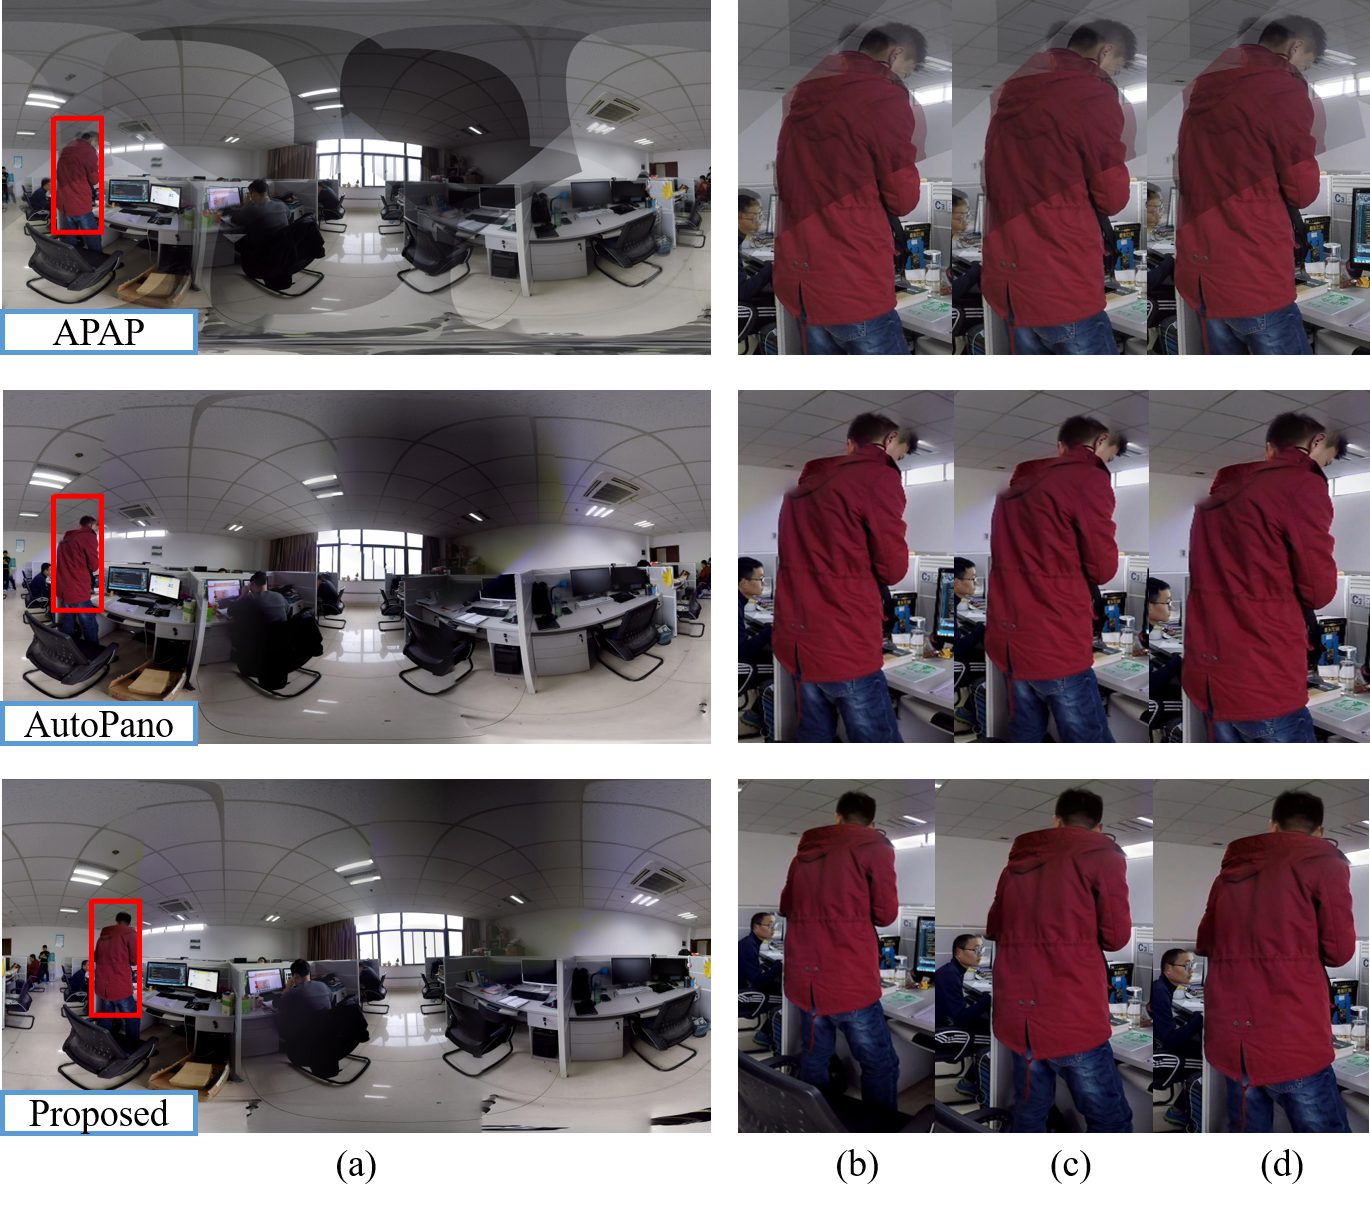
\includegraphics[scale=0.38]{picture38.png}
\caption{Comparisons with APAP, AutoPano and our method when there is an object moving in the overlapped region. From left to right: (a) one of the stitched frames, (b) enlarged views of local
detail in frame $t_1$, (c) enlarged views of local detail in frame $t_2$, (d) enlarged views of local detail in frame $t_3$.}
\label{fig:more2}
\end{figure}
%\section*{References}

%\begin{thebibliography}{00}
%\bibitem{b1} G. Eason, B. Noble, and I. N. Sneddon, ``On certain integrals of Lipschitz-Hankel type involving products of Bessel functions,'' Phil. Trans. Roy. Soc. London, vol. A247, pp. 529--551, April 1955.
%\bibitem{b2} J. Clerk Maxwell, A Treatise on Electricity and Magnetism, 3rd ed., vol. 2. Oxford: Clarendon, 1892, pp.68--73.
%\bibitem{b3} I. S. Jacobs and C. P. Bean, ``Fine particles, thin films and exchange anisotropy,'' in Magnetism, vol. III, G. T. Rado and H. Suhl, Eds. New York: Academic, 1963, pp. 271--350.
%\bibitem{b4} K. Elissa, ``Title of paper if known,'' unpublished.
%\bibitem{b5} R. Nicole, ``Title of paper with only first word capitalized,'' J. Name Stand. Abbrev., in press.
%\bibitem{b6} Y. Yorozu, M. Hirano, K. Oka, and Y. Tagawa, ``Electron spectroscopy studies on magneto-optical media and plastic substrate interface,'' IEEE Transl. J. Magn. Japan, vol. 2, pp. 740--741, August 1987 [Digests 9th Annual Conf. Magnetics Japan, p. 301, 1982].
%\bibitem{b7} M. Young, The Technical Writer's Handbook. Mill Valley, CA: University Science, 1989.
%\end{thebibliography}
%\vspace{12pt}
%\color{red}
%IEEE conference templates contain guidance text for composing and formatting conference papers. Please ensure that all template text is removed from your conference paper prior to submission to the conference. Failure to remove the template text from your paper may result in your paper not being published.

\end{document}
